 % Slides- Statins, RD results
% Update: 12/09/23
% ---------------------------------- Setup --------------------------------- %
\documentclass[aspectratio=169,12pt]{beamer}

\usepackage[utf8]{inputenc}
\usepackage{amsmath}
\usepackage{tikz}
\usepackage{pgfplots}
\usepackage{graphicx}
\usepackage{hyperref}
\usepackage{xcolor}
\usepackage{accents}
\usepackage{amssymb}
\usepackage{mathtools}
\usepackage{booktabs,caption,subcaption,dcolumn}
\usepackage{multirow}
\usepackage[authoryear,round]{natbib}
\usepackage{rotating} % Rotating table
\usepackage{makecell} %multiline headers in tables 

% FixMe sticky editing notes
% to put the notes in, change "status=draft"
% to take notes out, change "status=final"
\usepackage[status=draft,inline,index]{fixme}
\fxsetup{theme=color,margin=false,mode=multiuser}

% Change font
\usepackage[default]{lato}
% \usefonttheme{serif}

% Wide-Itemize Environment
\newenvironment{wideitemize}
{\itemize\addtolength{\itemsep}{6pt}}{\enditemize}
\newenvironment{wideishitemize}{\itemize\addtolength{\itemsep}{4pt}}{\enditemize}

% colors
\definecolor{blue}{RGB}{70,50,170}
\definecolor{red}{RGB}{200,100,100}
\definecolor{yellow}{RGB}{240,200,100}
\definecolor{green}{RGB}{0,150,100}
\definecolor{purple}{RGB}{100,50,100}

% beamer colors
\setbeamercolor{frametitle}{fg=blue}
\setbeamercolor{title}{fg=blue}
\setbeamercolor{itemize item}{fg=blue}
\setbeamercolor{itemize subitem}{fg=blue}
\setbeamercolor{enumerate item}{fg=blue}
\setbeamercolor{enumerate subitem}{fg=blue}

% table of context colors
\setbeamercolor{section in toc}{fg=blue}
\setbeamercolor{subsection in toc}{fg=purple}
\setbeamersize{text margin left=1em,text margin right=1em} 

% to customized
\AtBeginSection[]{\begin{frame}[noframenumbering,plain]
		\frametitle{Outline}
		\tableofcontents[currentsection]
	\end{frame}}

% Add frame numbers
\setbeamertemplate{footline}[frame number]
%gets rid of bottom navigation symbols
\setbeamertemplate{navigation symbols}{}

% Transparency- pause
\setbeamercovered{transparent}

% regression stars
\newcommand{\starlegend}{$^{*}p<0.1$; $^{**}p<0.05$; $^{***}p<0.01$}

% for appendix
\usepackage{appendixnumberbeamer} 
\newcommand{\backupbegin}{
	\newcounter{framenumberappendix}
	\setcounter{framenumberappendix}{\value{framenumber}}
}
\newcommand{\backupend}{
	\addtocounter{framenumberappendix}{-\value{framenumber}}
	\addtocounter{framenumber}{\value{framenumberappendix}} 
}

\vfuzz=30pt
\title[]{\large WFH UK: \\
Meetings slides}


\subtitle[]{}

\date{\today}
\author[]{
Ori Nahshon Shoham
 }



\pgfplotsset{compat=1.16}

% ---------------------------------- Title Page --------------------------------- %
\begin{document}
\begin{frame}[noframenumbering,plain]
\titlepage
\end{frame}


% ---------------------------------- Intro --------------------------------- %
\section*{Introduction}

\begin{frame}{Current group definitions}
    \begin{itemize}
        \item Currently identify 3 groups of key workers (health, public safety and education) based on coarse industry and occupation at 2019.
        \item Other keyworker sectors include Key public services, Local and national government, Food and other necessary goods, Transport, "Utilities, communications and financial services"
        \item Shutdown sector based on coarse industry at 2019 and IFS definition
    \end{itemize}
\end{frame}
\begin{frame}{}
    \begin{figure}
        \centering
        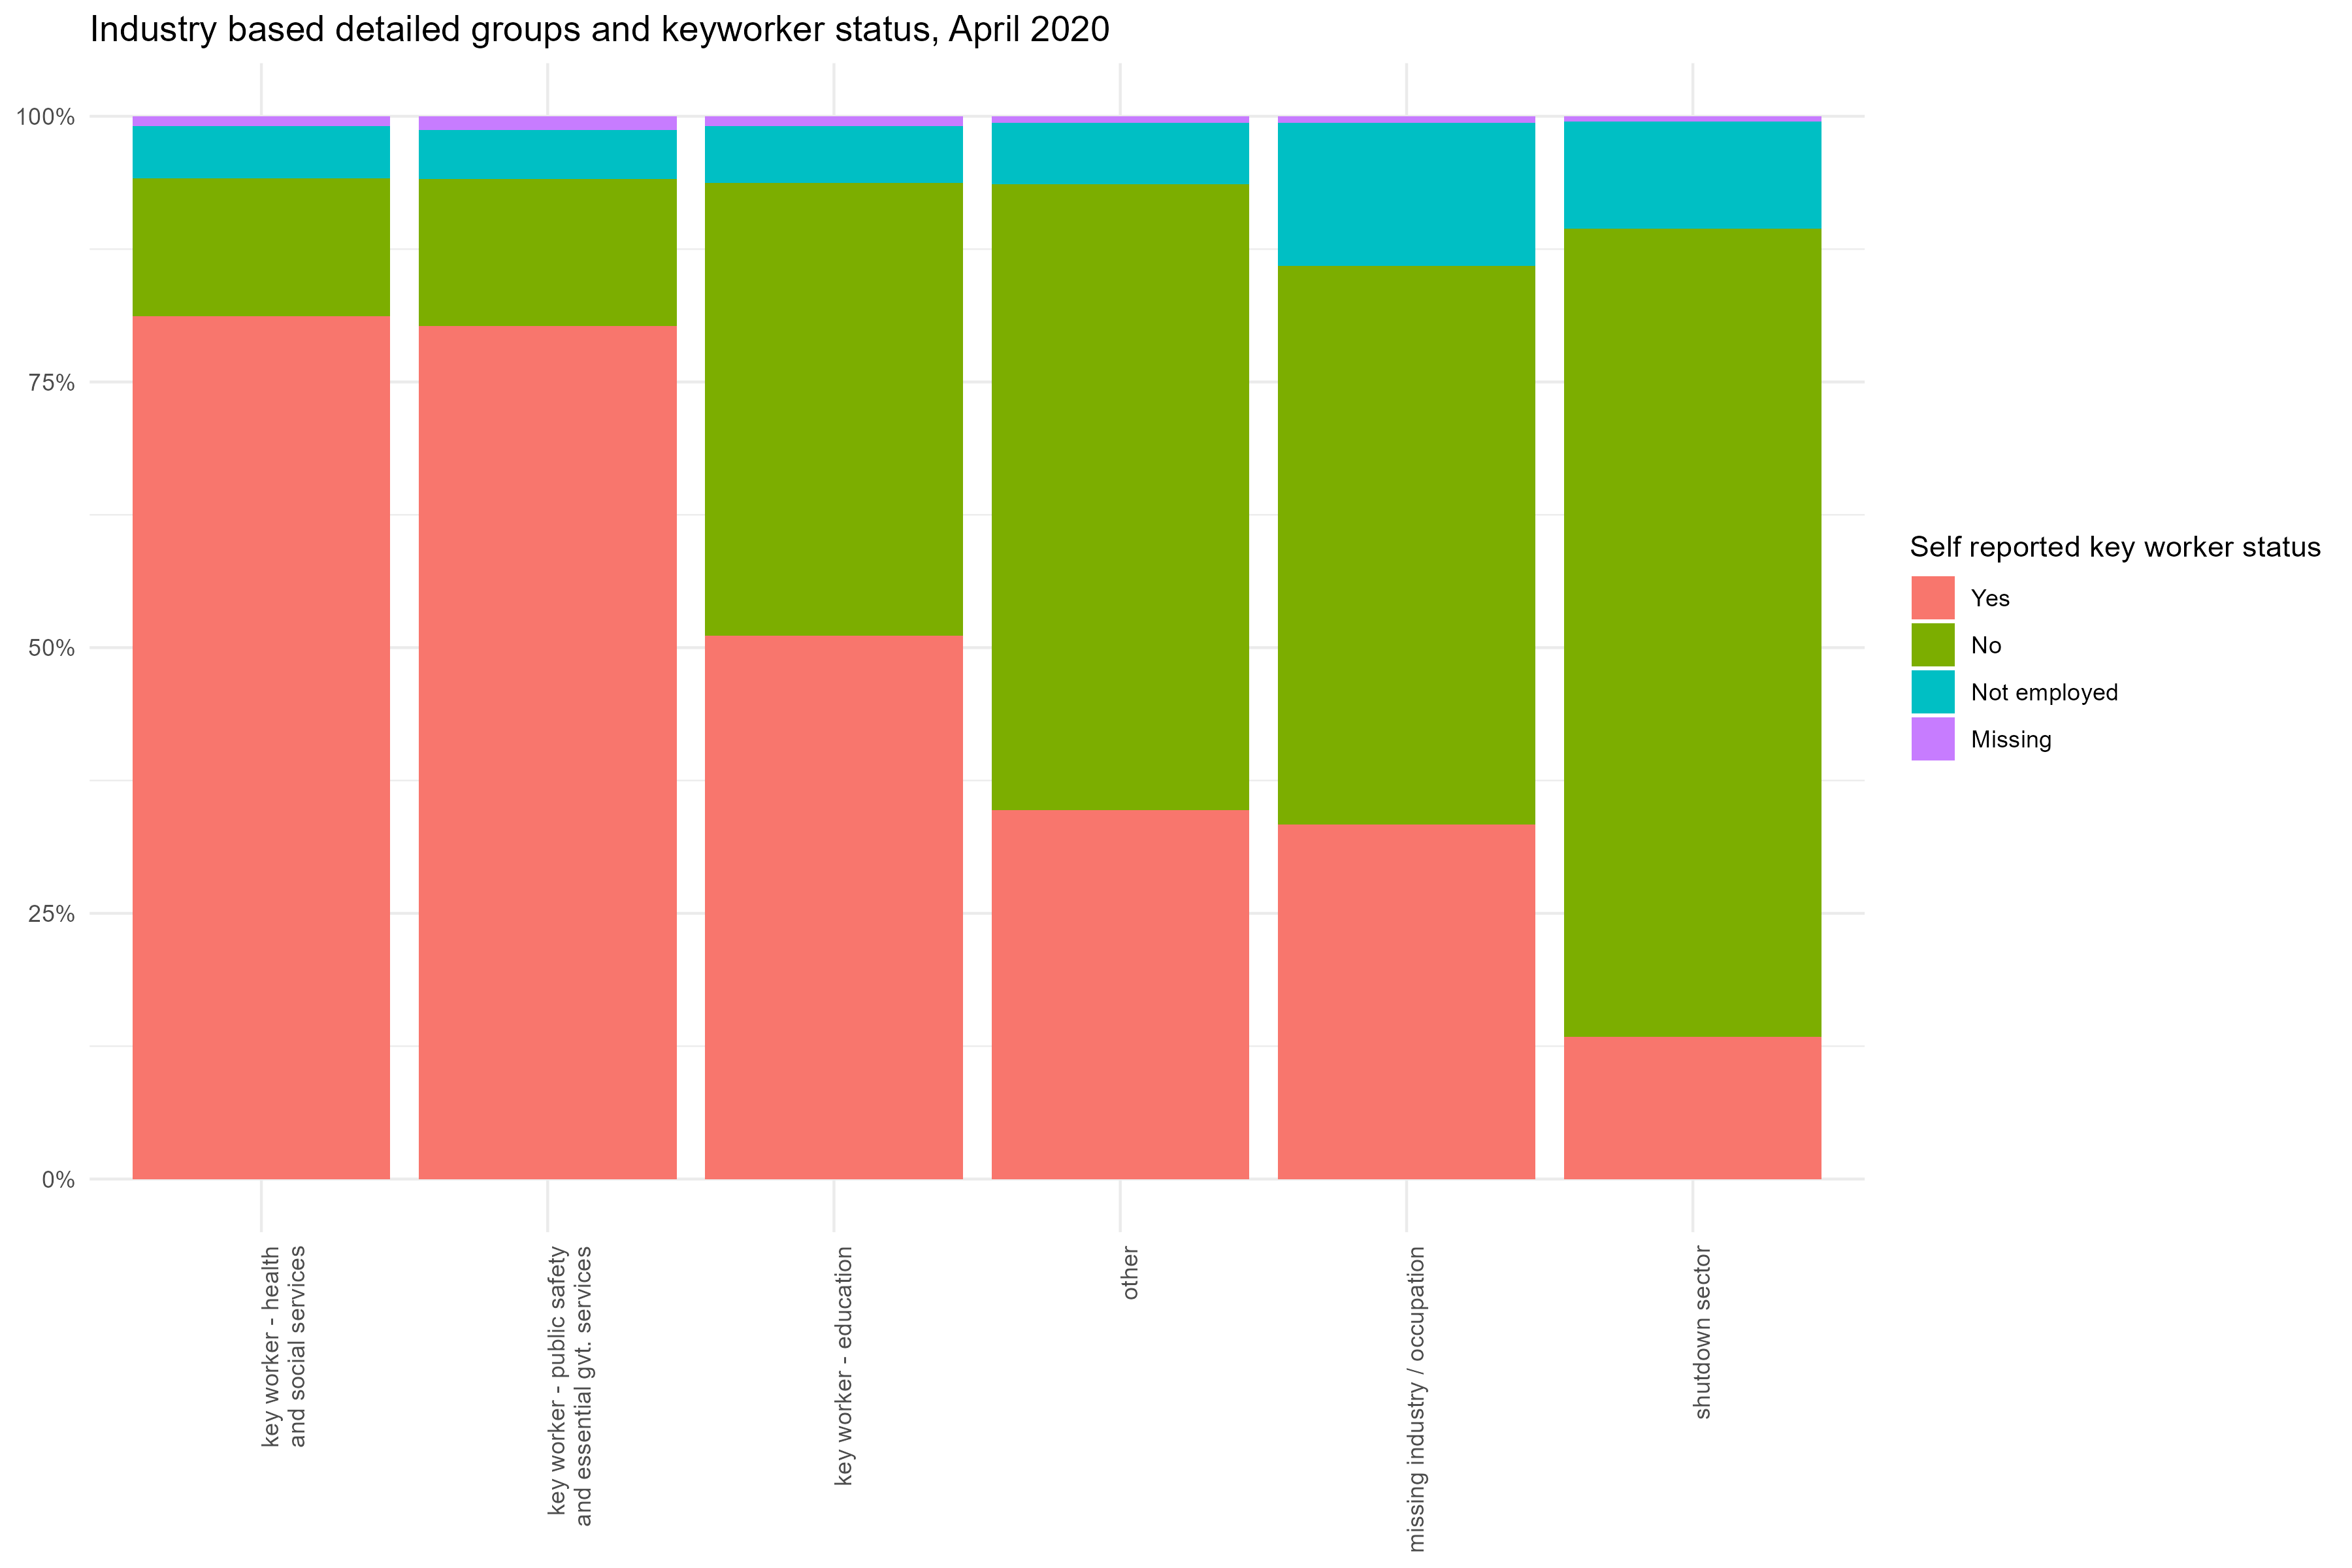
\includegraphics[width=0.85\linewidth]{figures/keyworker_def_explore_detailed_groups_april20.png}
    \end{figure}
\end{frame}
\begin{frame}{}
    \begin{figure}
        \centering
        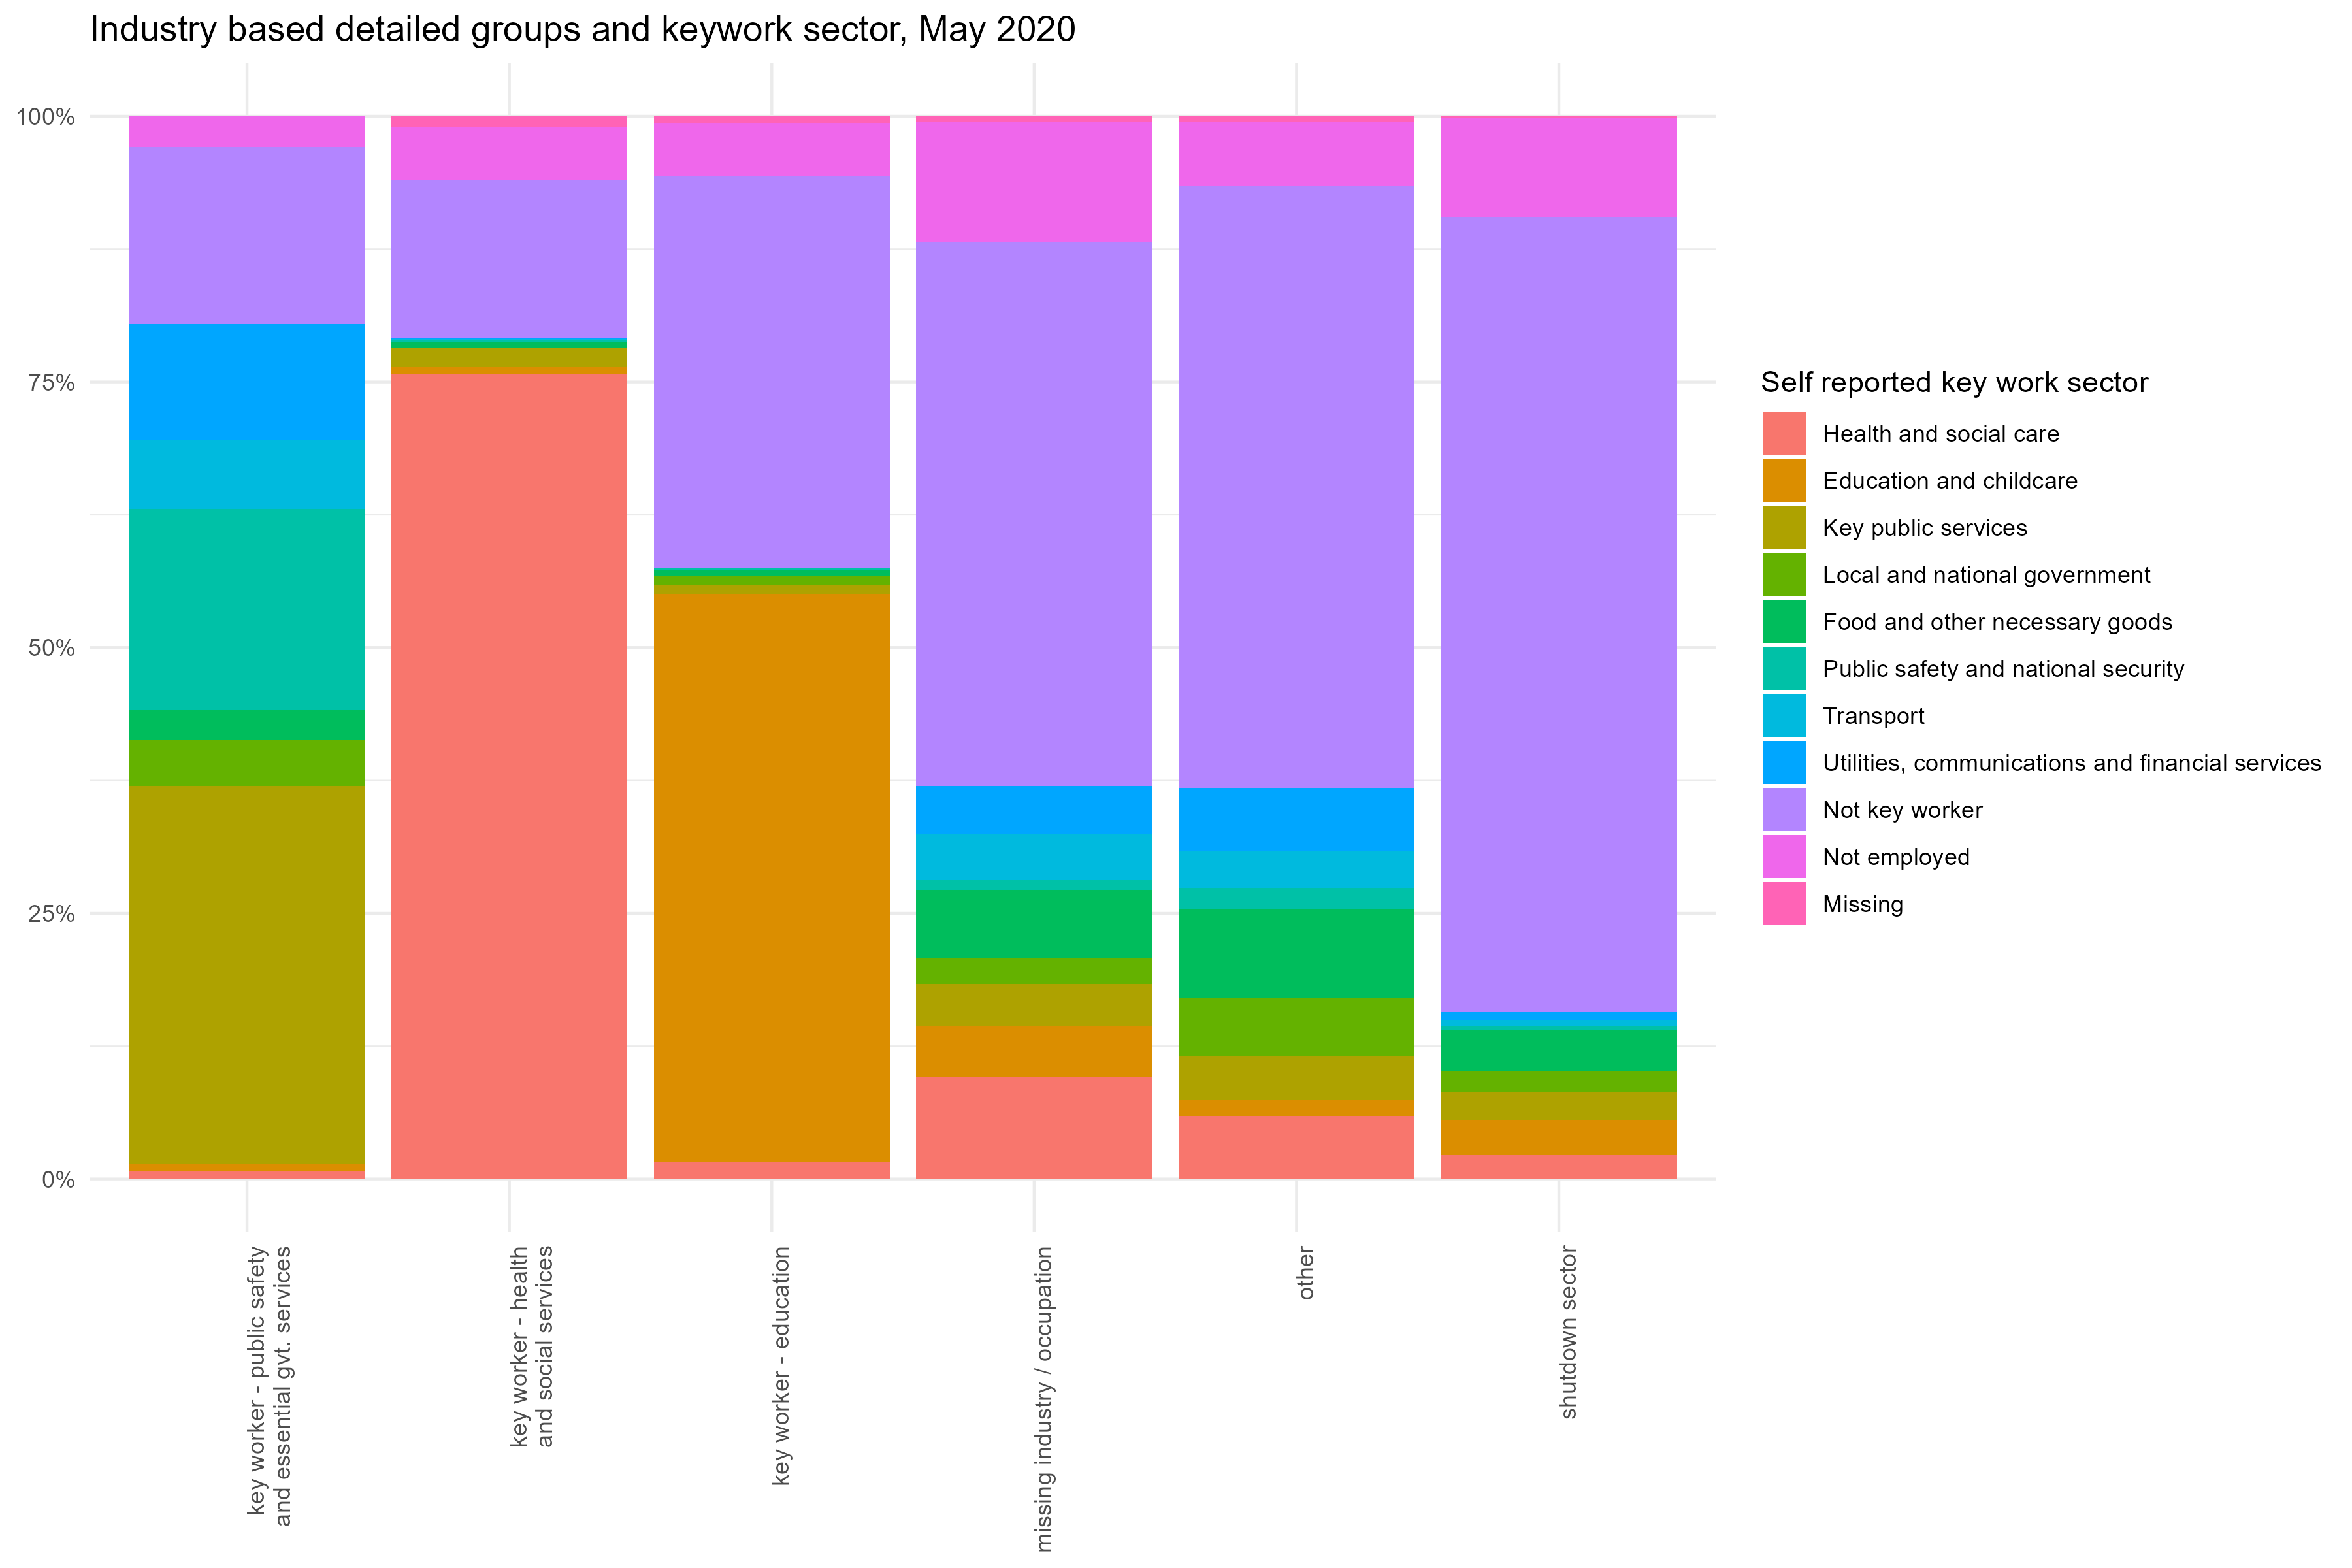
\includegraphics[width=0.85\linewidth]{figures/keywork_sector_def_explore_detailed_groups_may20.png}
    \end{figure}
\end{frame}
\begin{frame}{}
    \begin{figure}
        \centering
        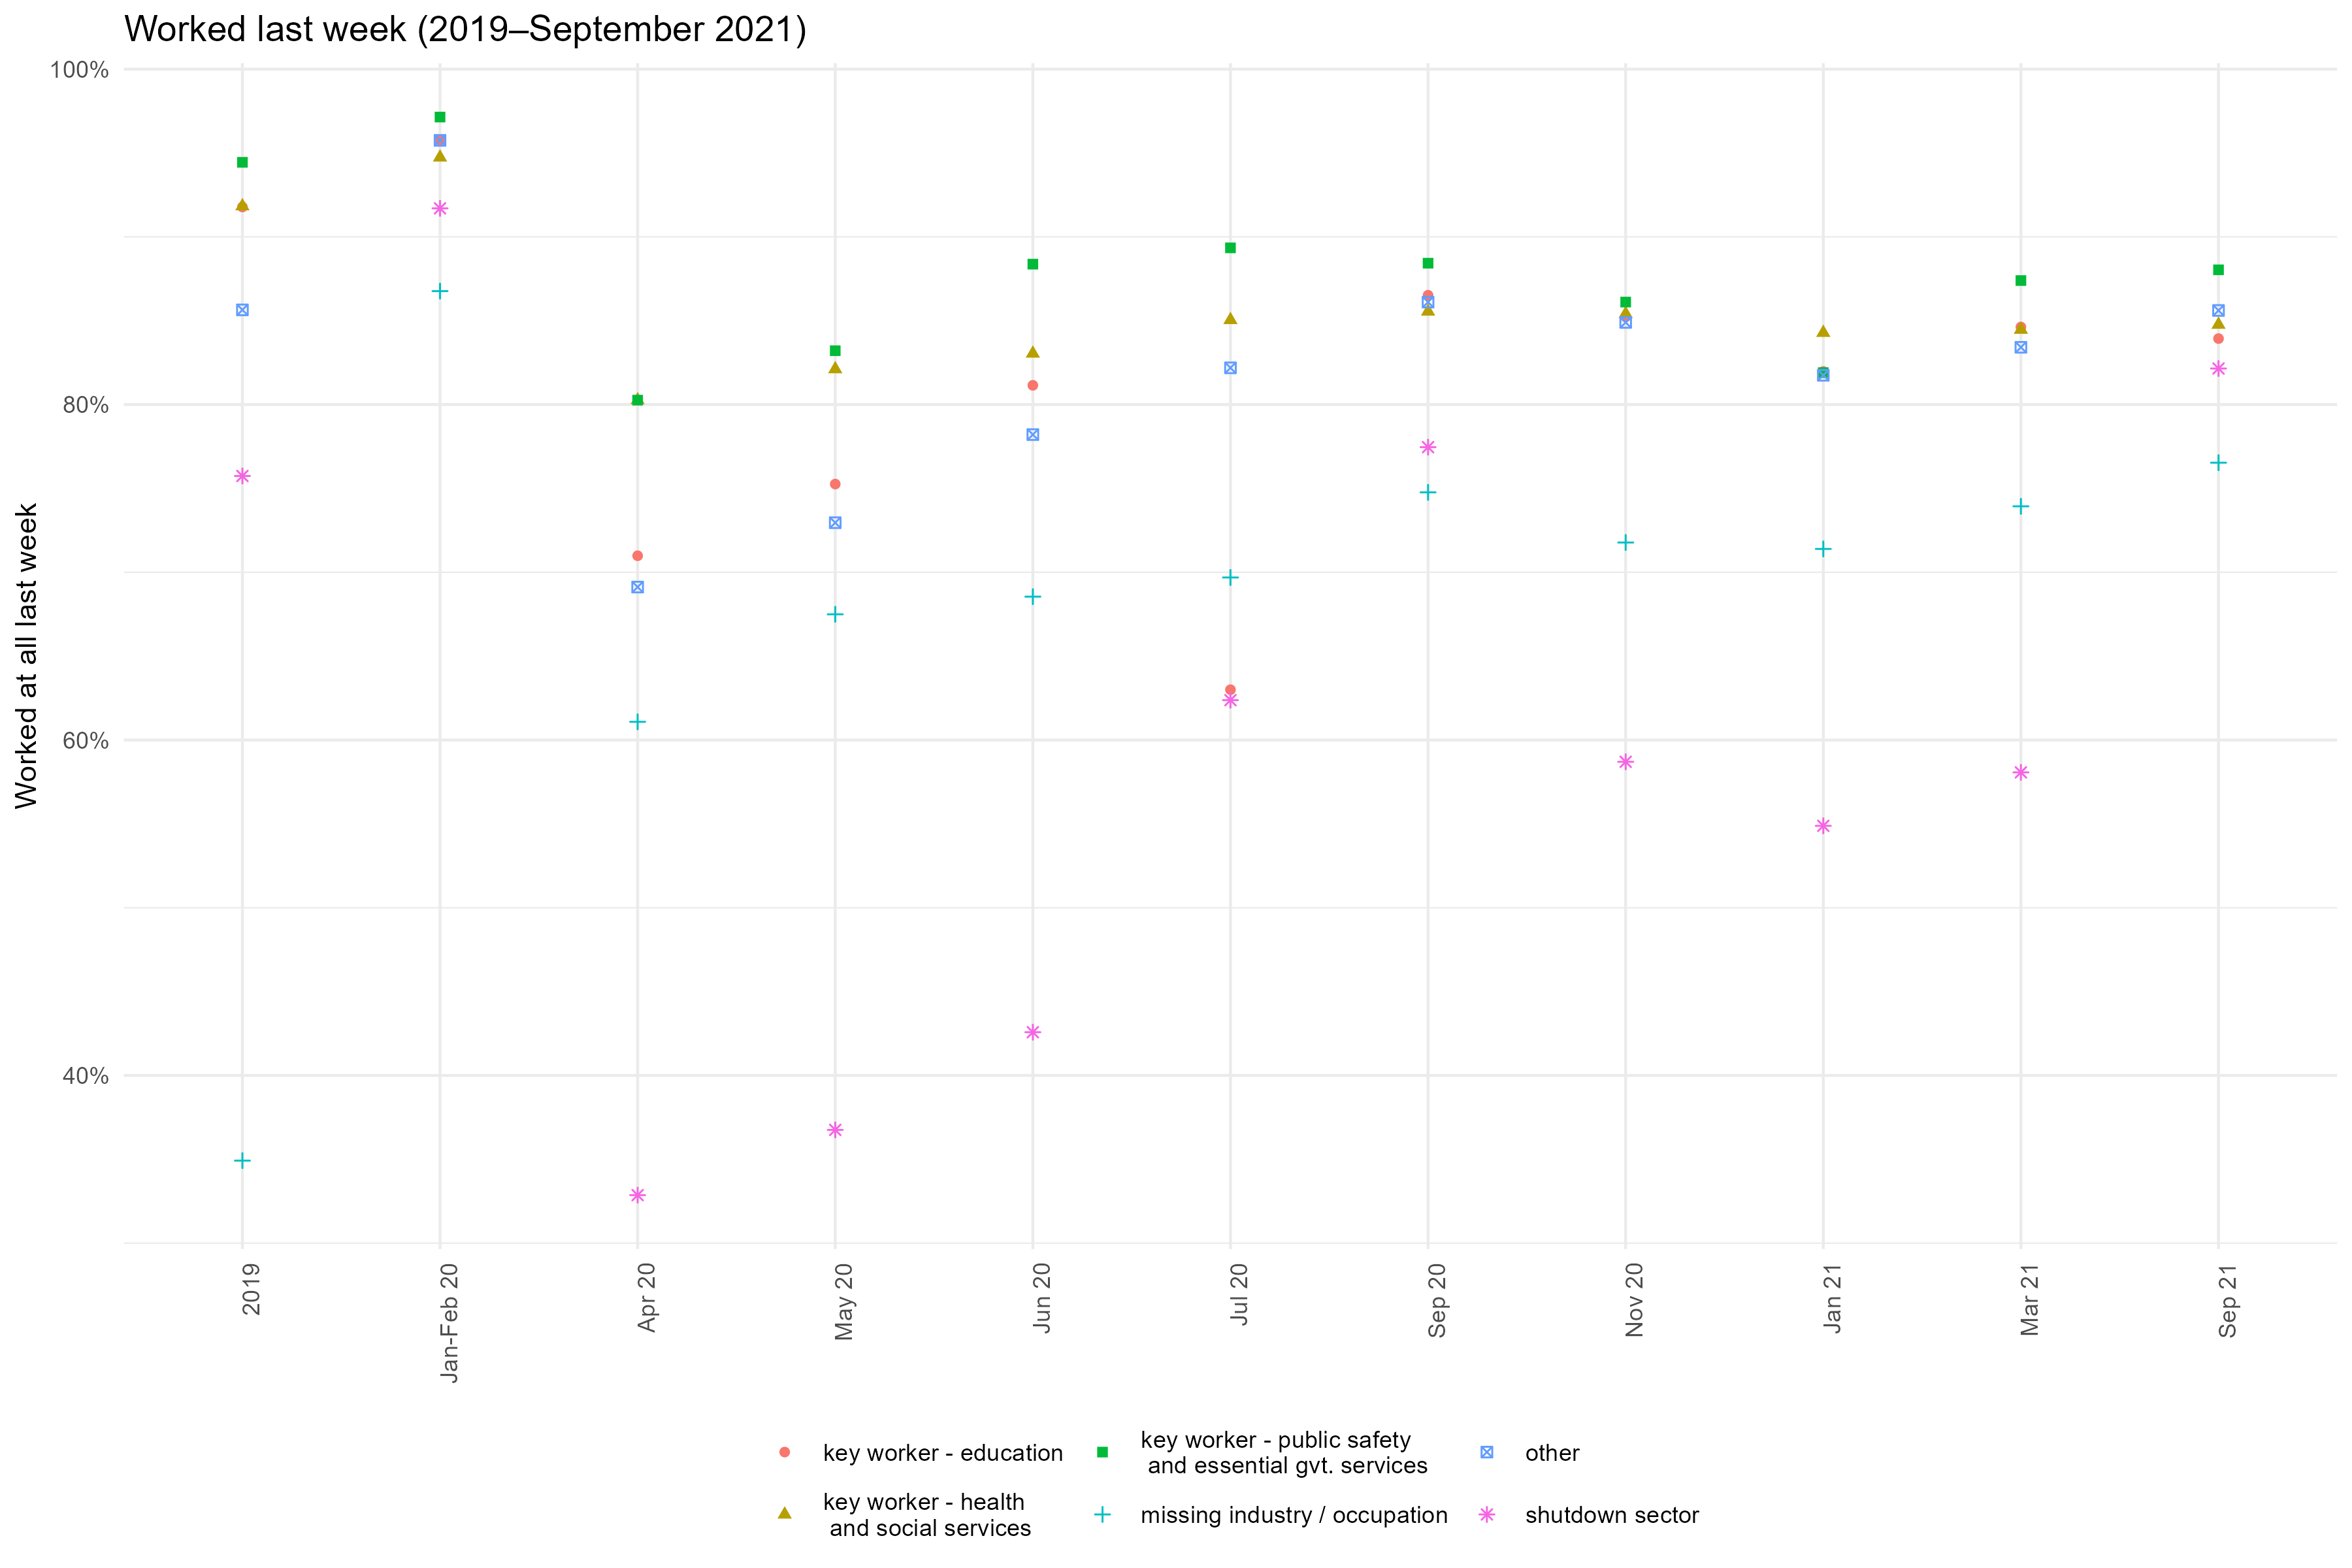
\includegraphics[width=0.85\linewidth]{figures/worked_at_all_detailed_groups_overtime.png}
    \end{figure}
\end{frame}

\begin{frame}{}
    \begin{figure}
        \centering
        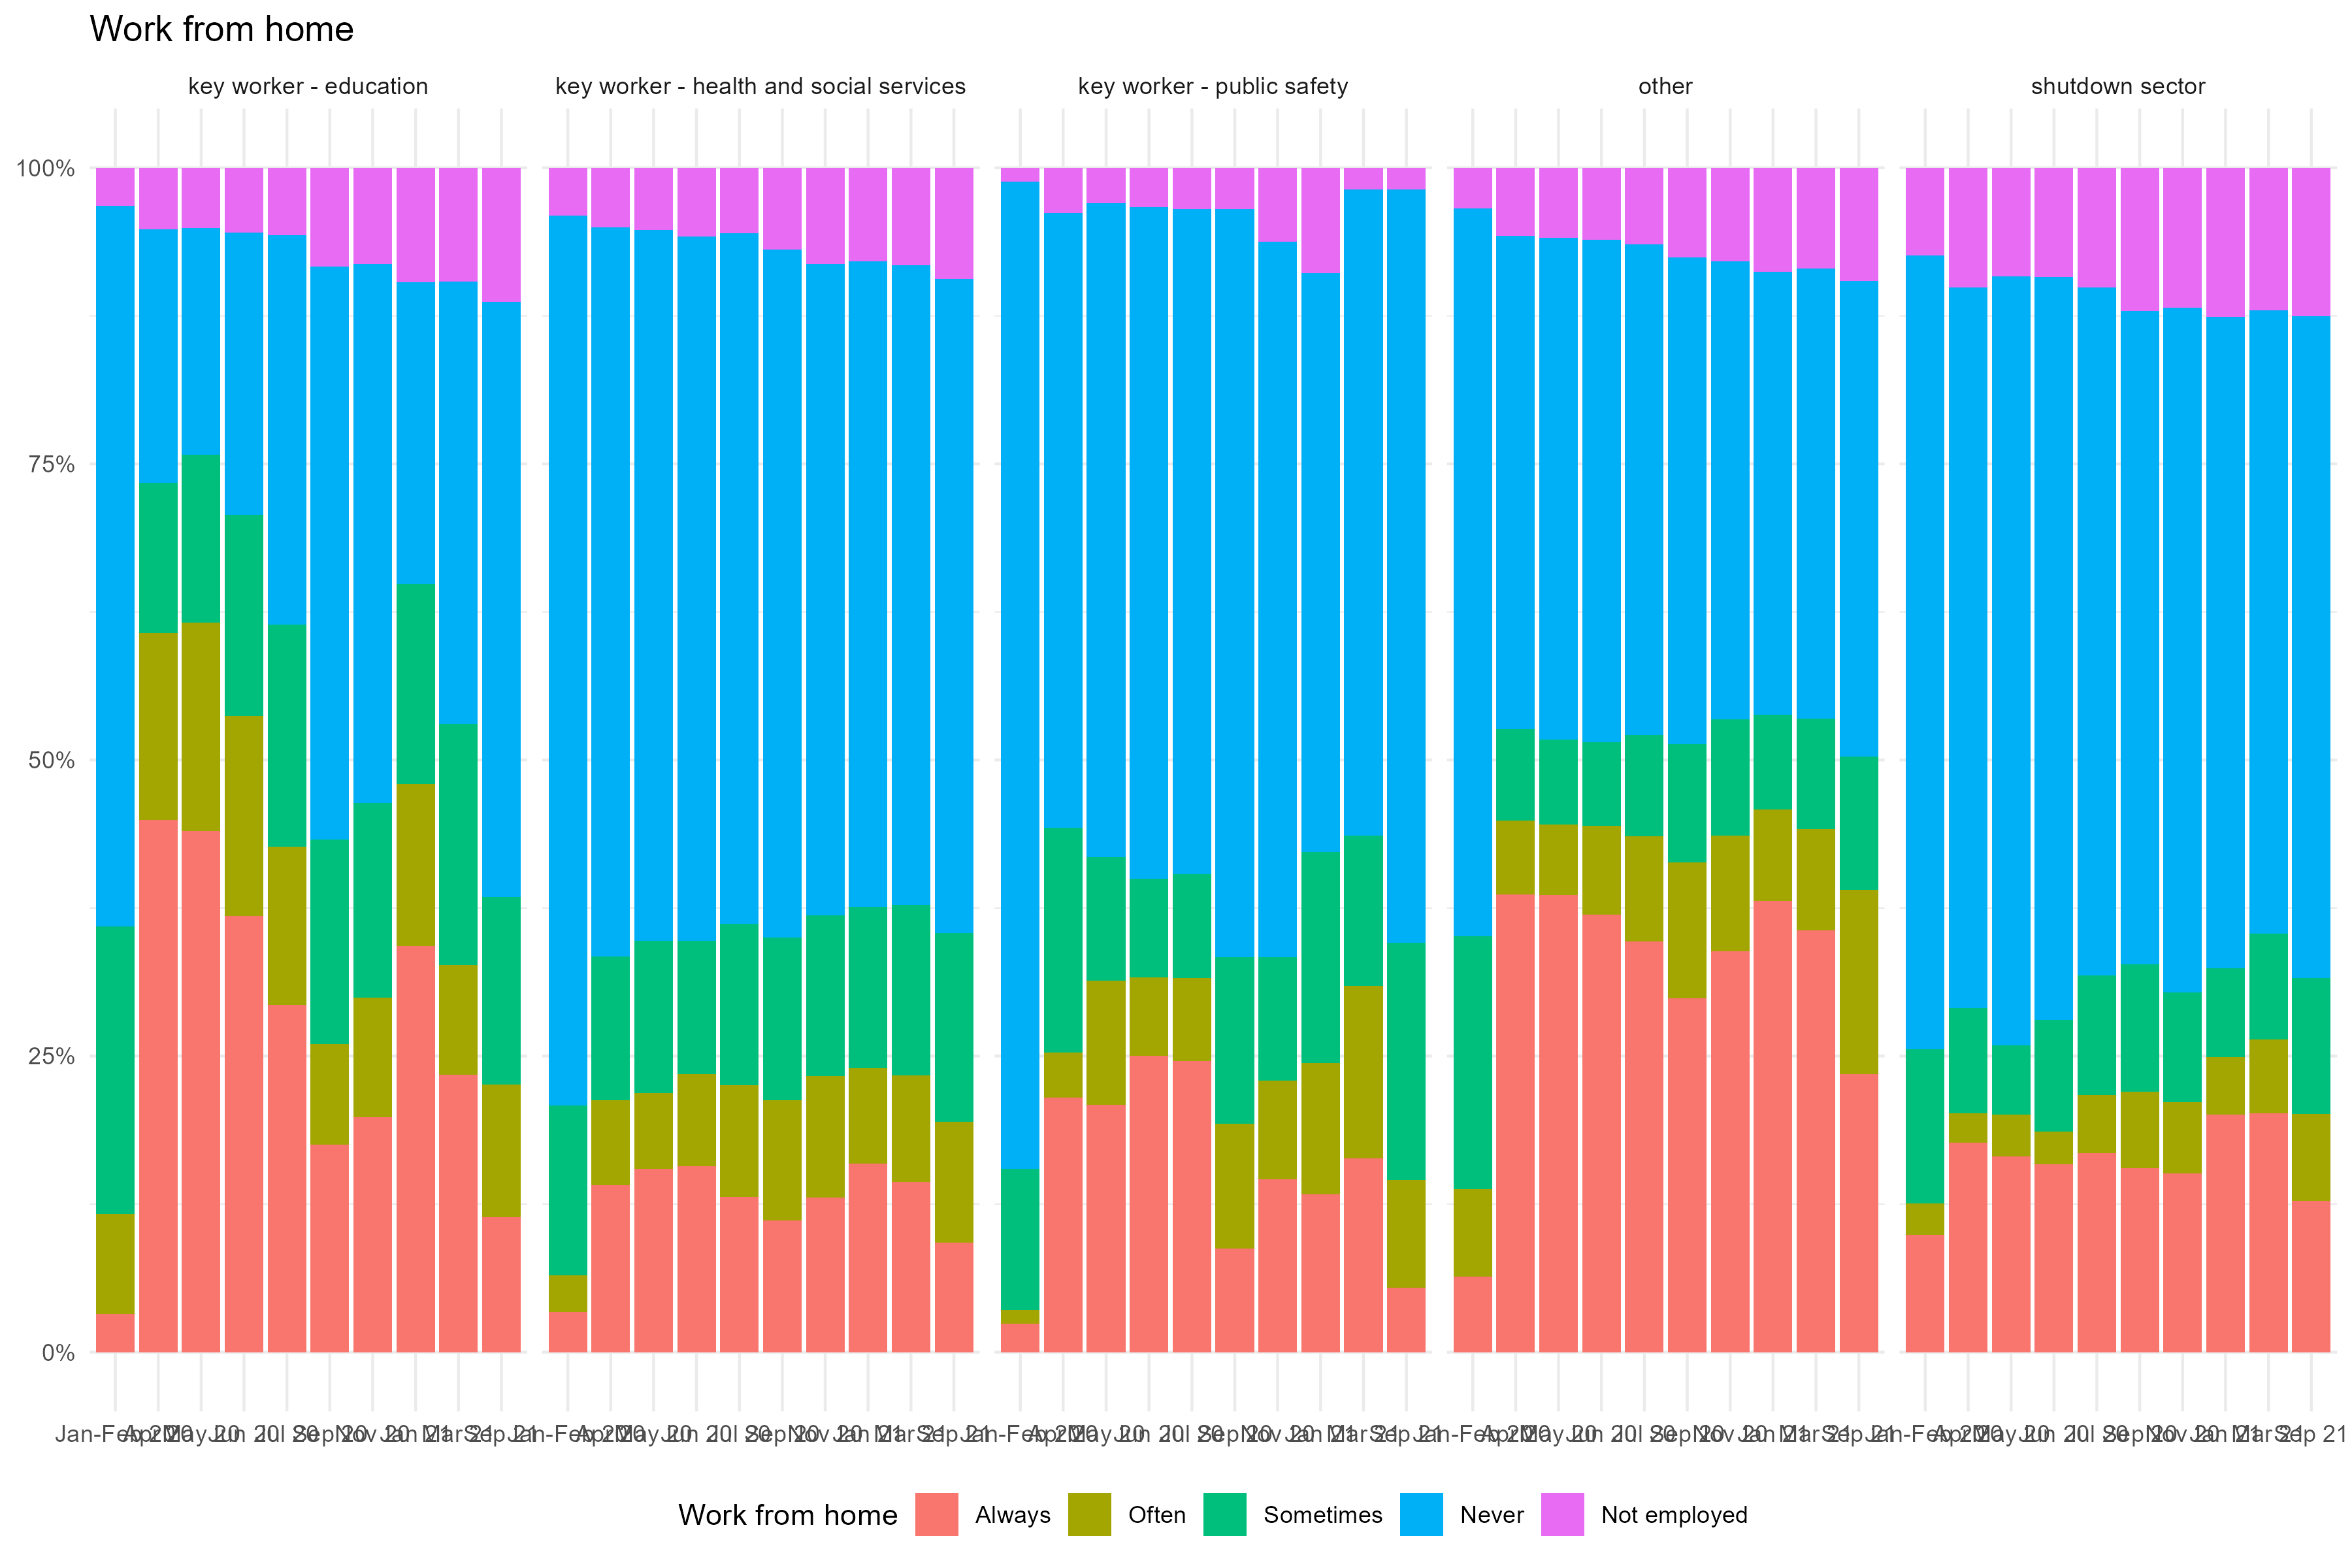
\includegraphics[width=0.85\linewidth]{figures/wfh_detialed_groups_overtime.png}
    \end{figure}
\end{frame}

\begin{frame}{}
    \begin{figure}
        \centering
        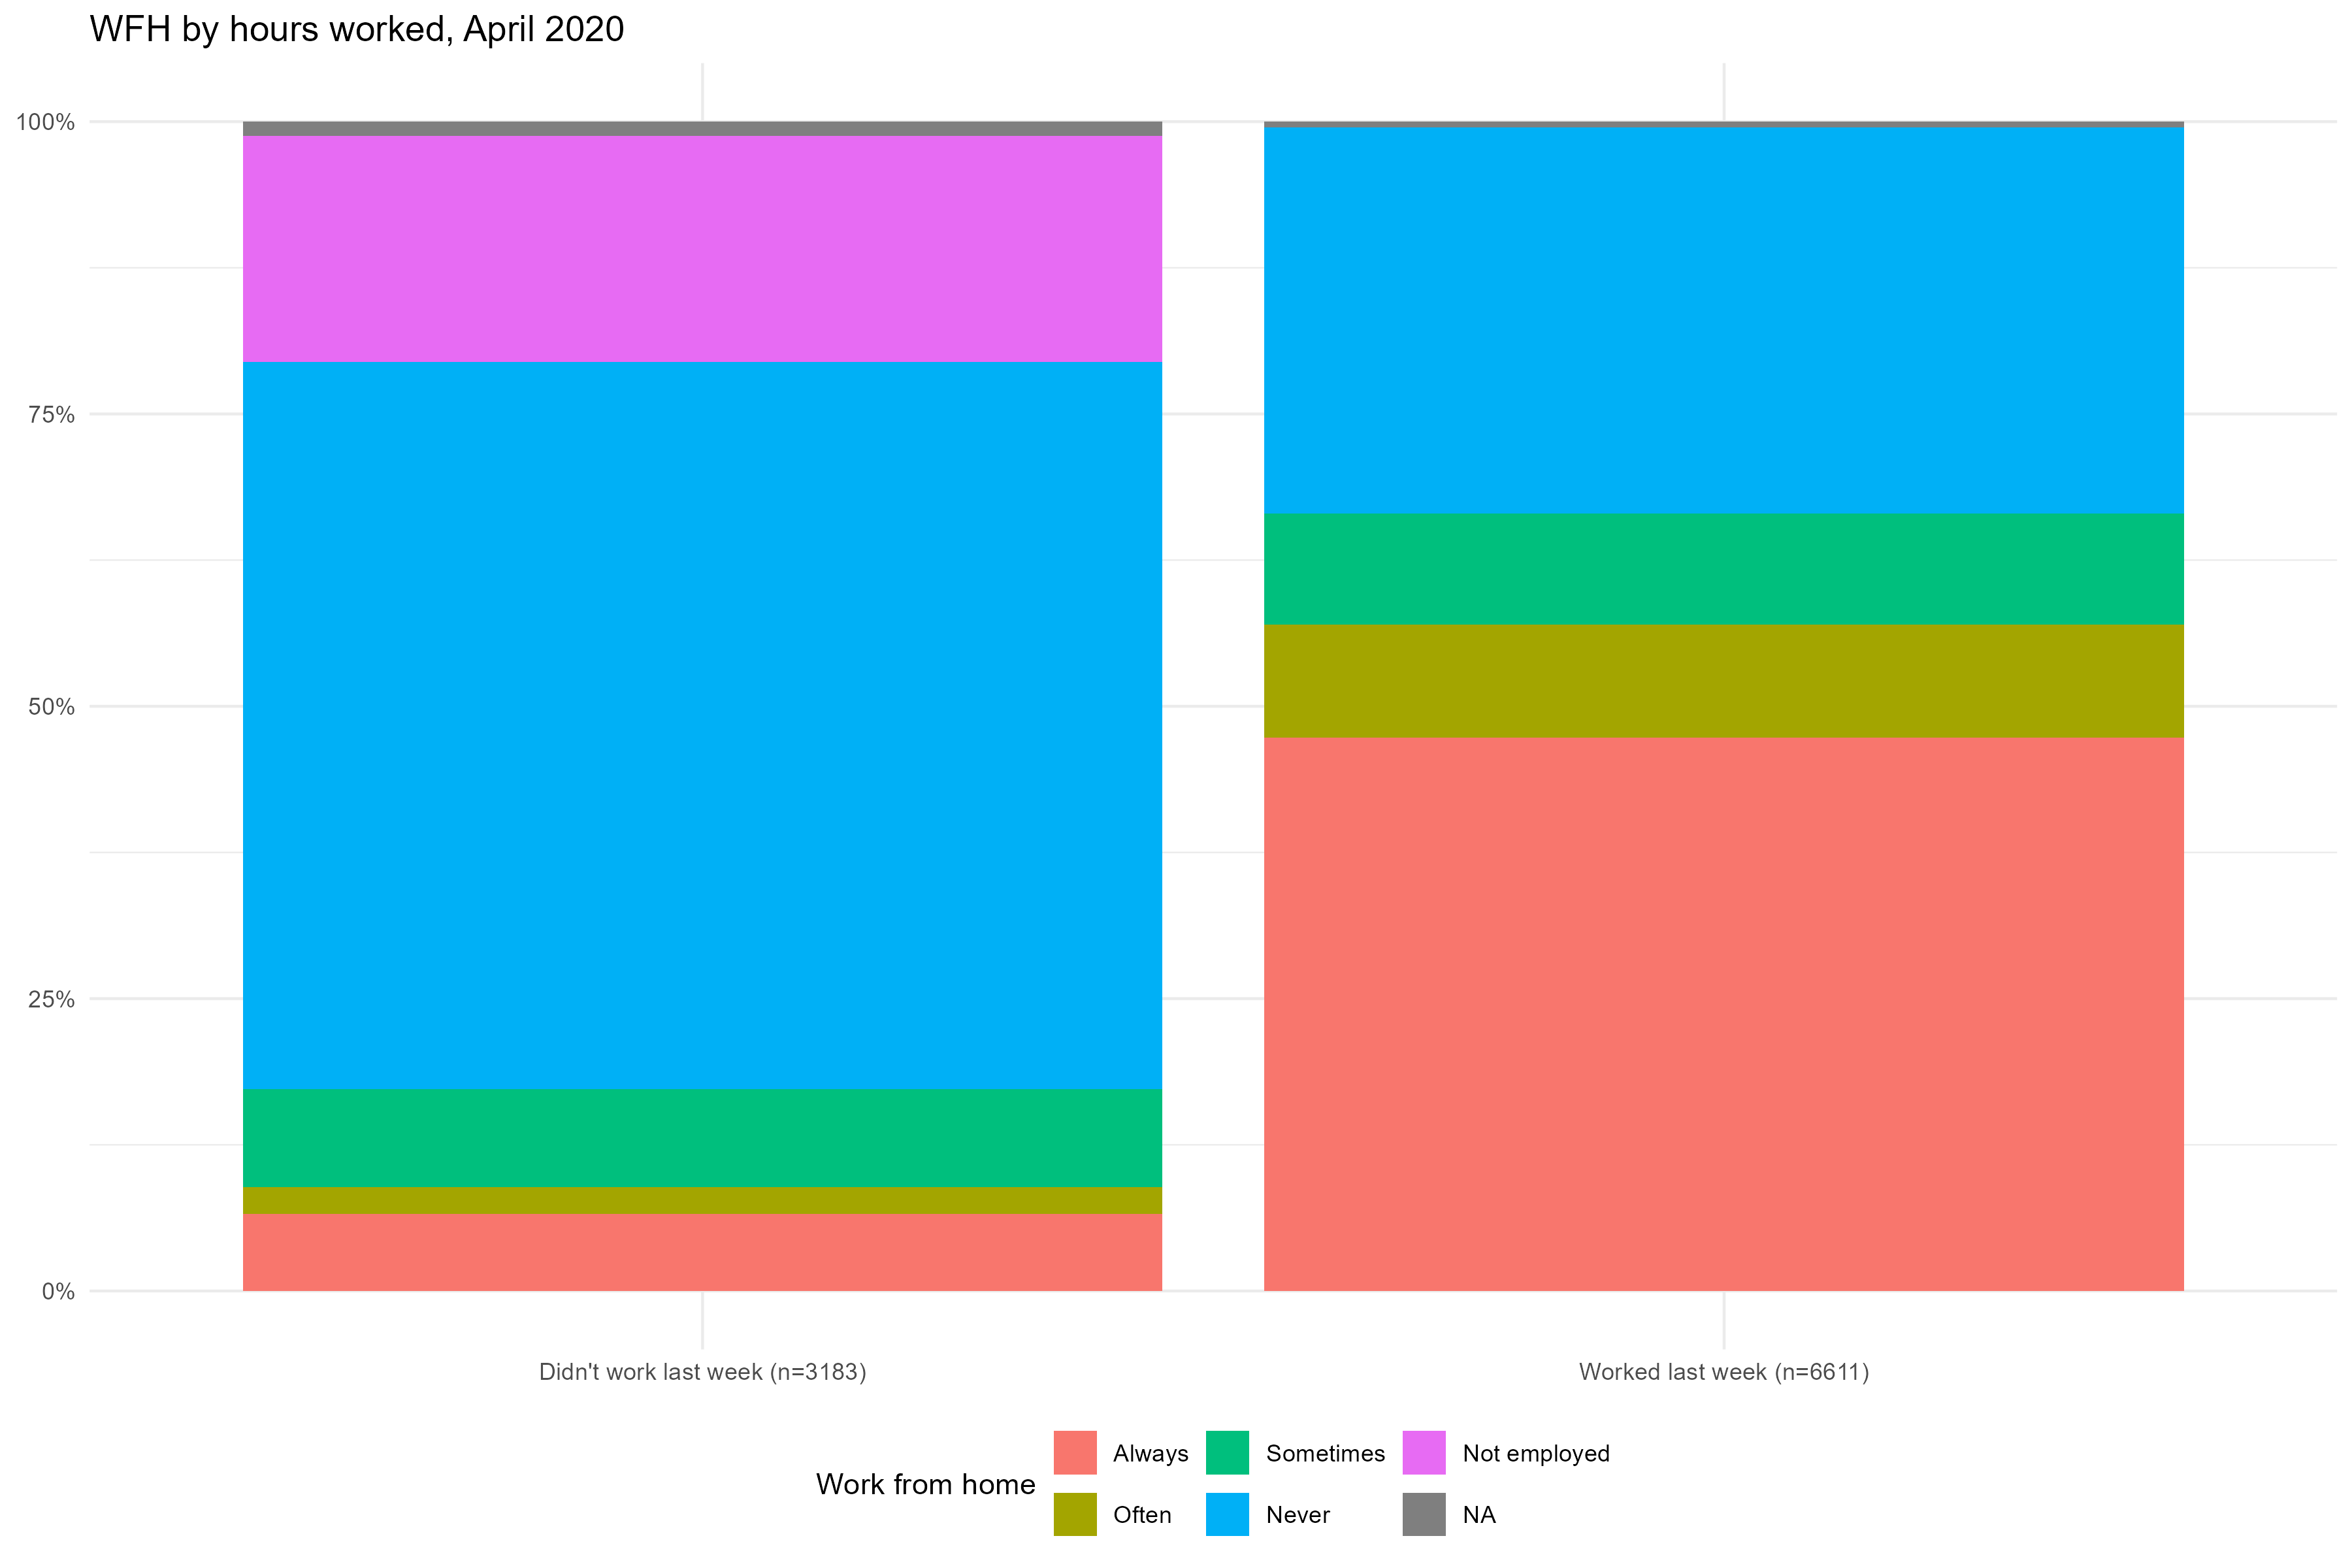
\includegraphics[width=0.85\linewidth]{figures/worked_at_all_wfh_april20.png}
    \end{figure}
\end{frame}
\begin{frame}{Work outside definition}
    \begin{itemize}
        \item Currently define $workoutside_i = 1$ if worked positive hours last week and not always working from home (NA if does not answer work status or missing WFH answer)
    \end{itemize}
\end{frame}
\begin{frame}{}
        \begin{figure}
        \centering
        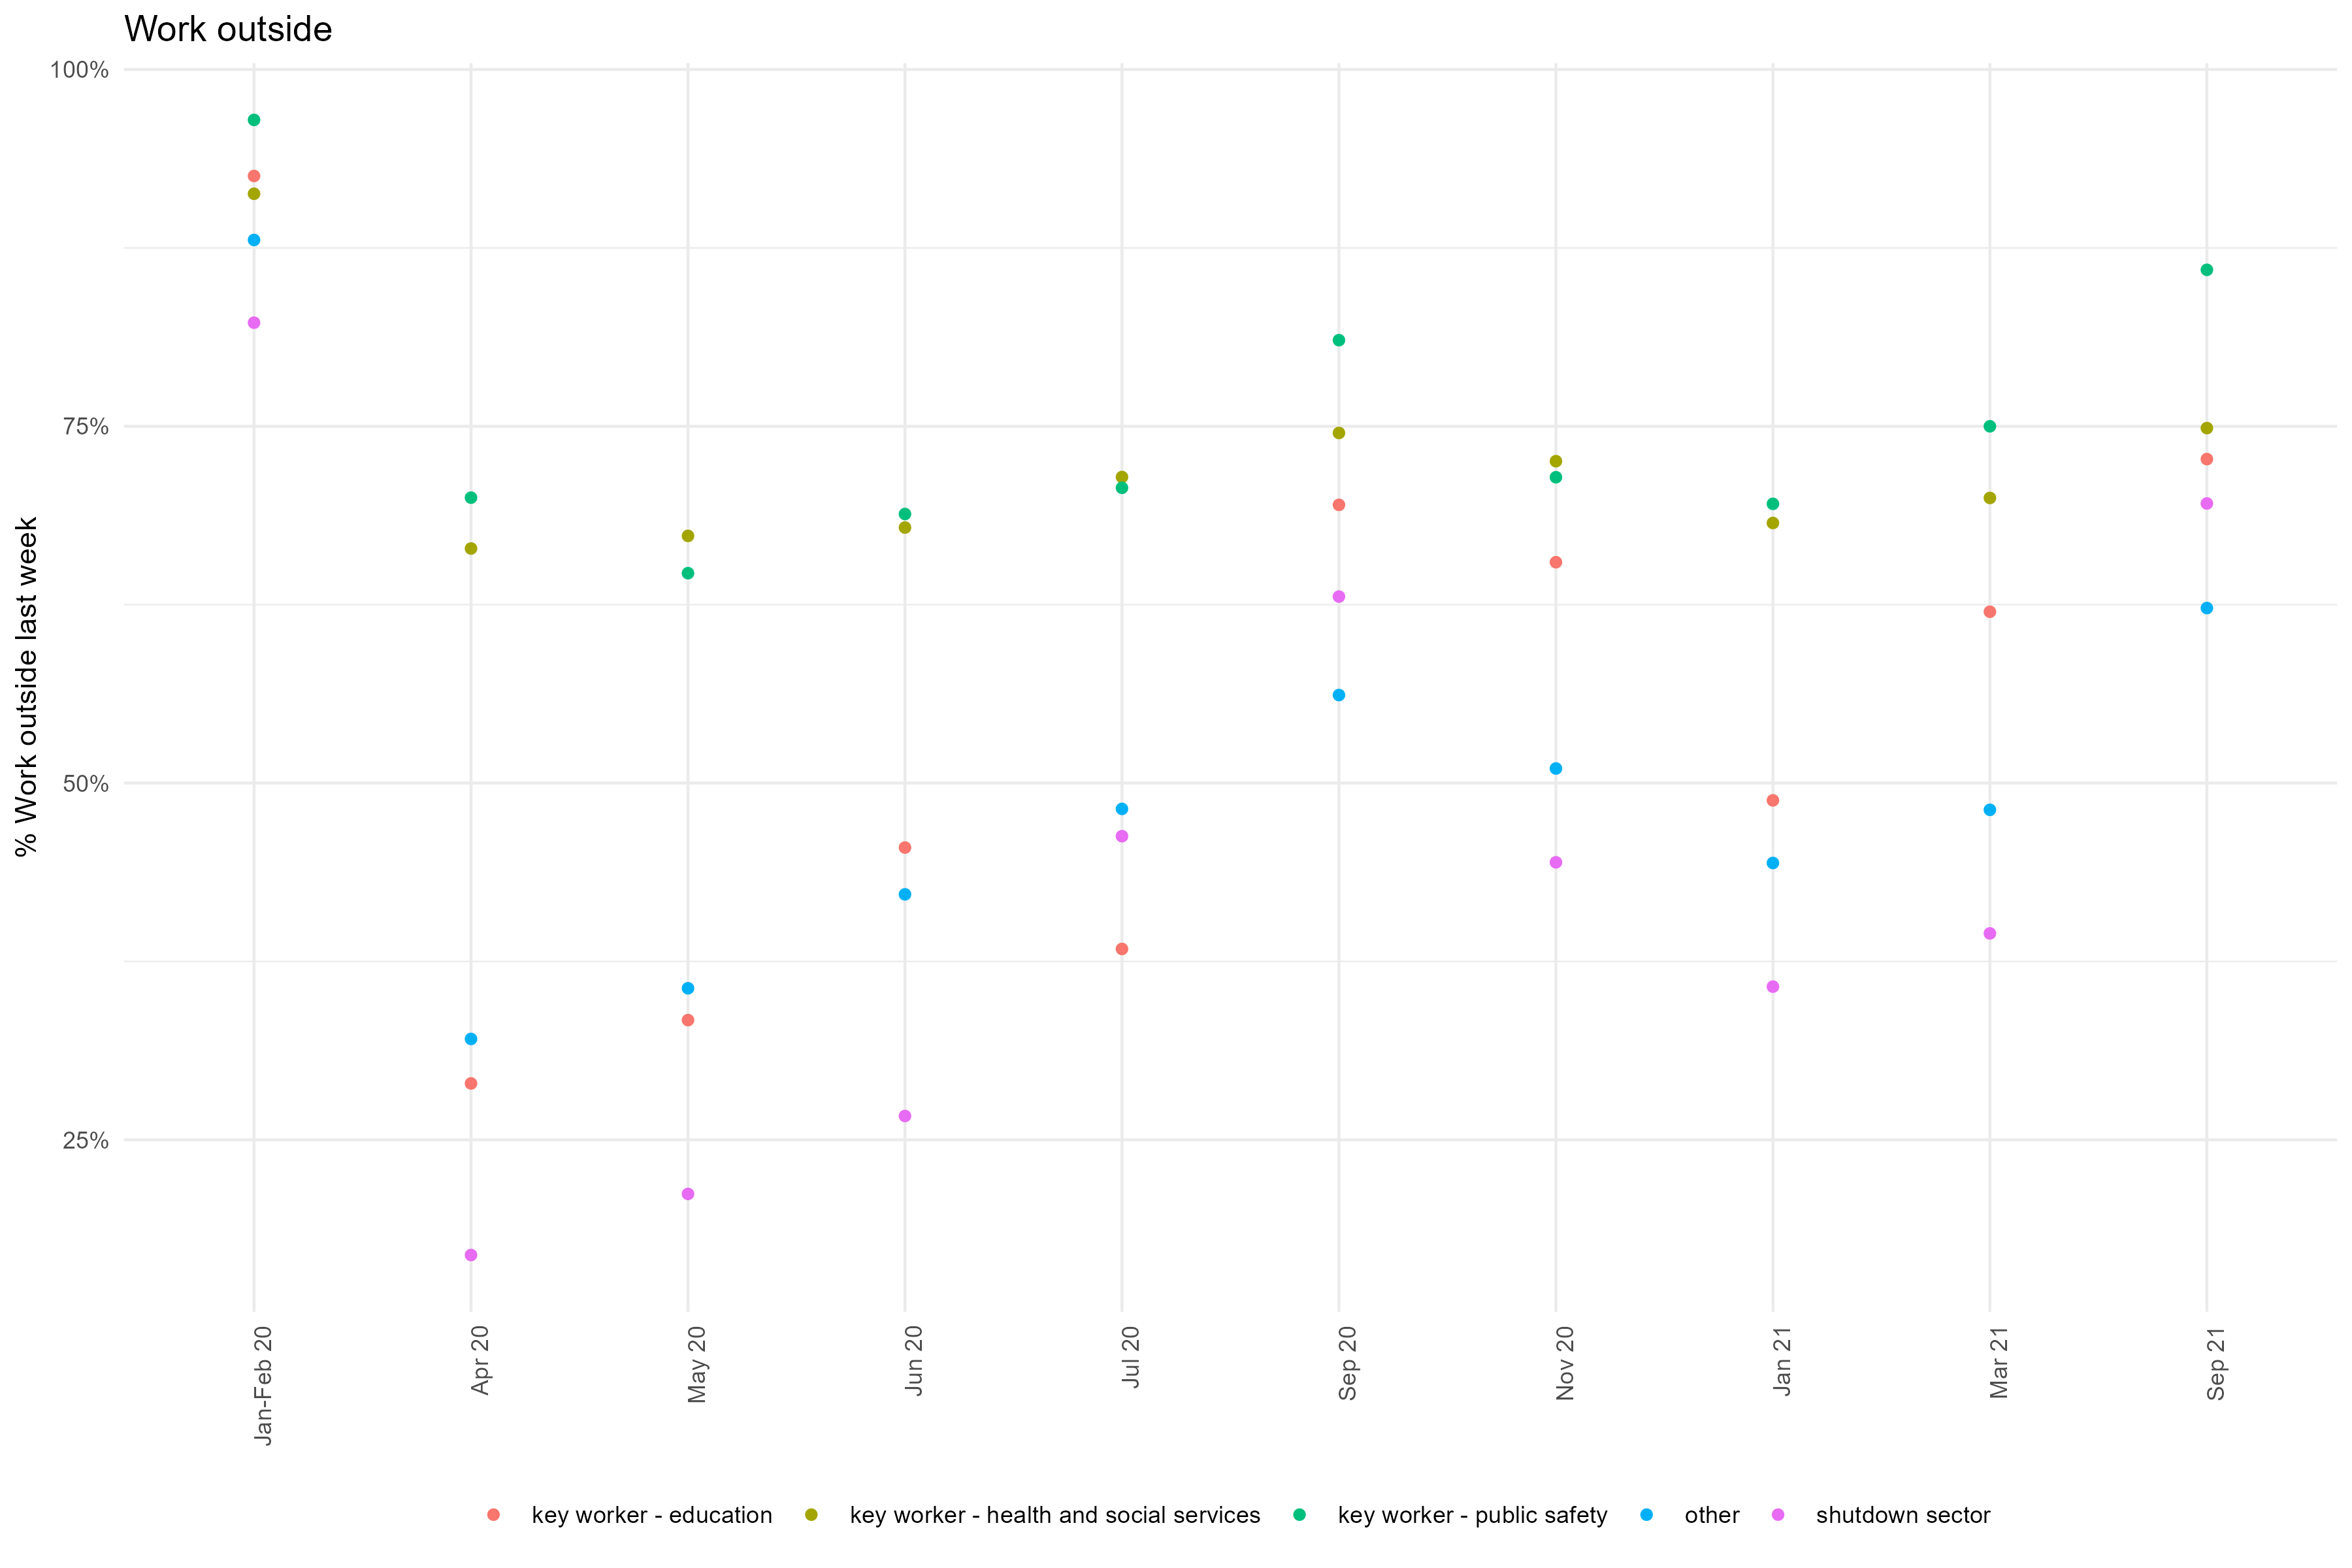
\includegraphics[width=0.85\linewidth]{figures/workoutside_overtime_detailed_groups.png}
    \end{figure}
\end{frame}

\begin{frame}{Work outside}
    \begin{table}
\centering
\begin{talltblr}[         %% tabularray outer open
caption={Work Outside by Industry Group},
note{}={+ p \num{< 0.1}, * p \num{< 0.05}, ** p \num{< 0.01}, *** p \num{< 0.001}},
note{ }={Standard errors in parentheses. * p<0.10, ** p<0.05, *** p<0.01},
]                     %% tabularray outer close
{                     %% tabularray inner open
colspec={Q[]Q[]Q[]Q[]Q[]Q[]},
column{2,3,4,5,6}={}{halign=c,},
column{1}={}{halign=l,},
hline{12}={1,2,3,4,5,6}{solid, black, 0.05em},
}                     %% tabularray inner close
\toprule
& A & B & C & D & E \\ \midrule %% TinyTableHeader
Intercept & \num{0.359}*** & \num{0.321}*** & \num{0.283}* & \num{0.246} & \num{0.341}* \\
& (\num{0.028}) & (\num{0.006}) & (\num{0.138}) & (\num{0.244}) & (\num{0.168}) \\
Key – education &  & \num{-0.031}* & \num{-0.008} & \num{-0.010} & \num{0.012} \\
&  & (\num{0.014}) & (\num{0.014}) & (\num{0.027}) & (\num{0.016}) \\
Key – health &  & \num{0.344}*** & \num{0.358}*** & \num{0.400}*** & \num{0.370}*** \\
&  & (\num{0.014}) & (\num{0.014}) & (\num{0.032}) & (\num{0.016}) \\
Key – public safety &  & \num{0.379}*** & \num{0.374}*** & \num{0.397}*** & \num{0.311}*** \\
&  & (\num{0.052}) & (\num{0.051}) & (\num{0.065}) & (\num{0.085}) \\
Shutdown sector &  & \num{-0.151}*** & \num{-0.153}*** & \num{-0.109}** & \num{-0.151}*** \\
&  & (\num{0.019}) & (\num{0.019}) & (\num{0.034}) & (\num{0.023}) \\
Num.Obs. & \num{9793} & \num{9793} & \num{9717} & \num{4152} & \num{5565} \\
R2 & \num{0.165} & \num{0.076} & \num{0.095} & \num{0.077} & \num{0.120} \\
Industry FE & \checkmark &  &  &  &  \\
Occupation FE & \checkmark &  &  &  &  \\
Age controls &  &  & \checkmark & \checkmark & \checkmark \\
Education controls &  &  & \checkmark & \checkmark & \checkmark \\
Sample & All & All & All & Males & Females \\
\bottomrule
\end{talltblr}
\end{table}


\end{frame}

\end{document}
% ---------------------------------- End --------------------------------- %


%